% Chapter 4
\chapter{Clustering activation patterns of spatially-referenced neurons}
\chaptermark{Clustering activation patterns of spatially-referenced neurons}

The previous approach only accounted for the analysis of calcium traces of individual neurons. The analysis of populations of neurons could only be performed as a second phase by combining the results of multiple analyses.
Although not ideal, this approach is sometimes the only viable option due to the complexity and the large size of the data as, for example, the length of the individual series in the Allen Brain Observatory data.

In this chapter we develop a model to analyze the activity of groups of neurons and to cluster this activity on the basis of recurring patterns of activation. As motivating application, we consider the hippocampal neurons data described in Section \ref{ch1_sec:hippoc_data}: differently from the Allen Brain Observatory data, here the animal is not subjected to different types of stimuli, and it is freely moving within an environment.
This type of experimental setting is often used to investigate hippocampal dynamics and connectivity patterns, which consist of groups of co-activating neurons. 
Hippocampal neurons underlying spatial navigation are thought to have a distributed organization, not strictly connected to the anatomical structure; however, many studies have shown that neurons with the same place field tuning often tend to neighbor one another~\parencite{Eichenbaum1989, Redish2001}. Hence, when investigating clusters of co-activating neurons, it can be relevant to take into account their spatial location and, in particular, their proximity to each other.
In particular, the interest is aimed to identifying subpopulations of neurons which share a common spiking activity over seconds-long periods of time \parencite{Bittner2017}. In the case of the data that we considered (recorded with a frequency of 15 frames per second), it means estimating clusters of temporal activity patterns with a duration up to a few hundreds of time points.

We develop a nonparametric mixture model that allows for simultaneous deconvolution of calcium traces and identification of groups of neurons with a similar pattern of activity during seconds-long periods. Moreover, the weights of the mixture prior are informed using the spatial proximity between cells. In particular, to identify such clusters, our modeling framework looks for similarities in the deconvolved binary time series describing the active/resting state of the neurons at each time point.
A possible difficulty in clustering these time series arises from the presence of isolated or erratic spikes, which make the observed series somehow different, even if the overall patterns match. To overcome this drawback, we perform clustering at a latent level through a process that describes, at each time point, the probability of observing a spike, hence allowing for some degree of discrepancy across series in the same cluster.


\section{Model and prior specification}
Once again, we employ the general model for the calcium dynamics introduced in equation~\eqref{ch1_eq:armodel} of Chapter 1. However, differently from the previous chapter, here we consider $n$ neurons, so we also introduce the index $i=1,\dots,n$ corresponding to each fluorescence trace. 
Moreover, we split the parameters $A_t$ of equation~\eqref{ch1_eq:armodel} into two separate components: $s_{i,t}\in\{0,1\}$ describing the presence/absence of a spike (the \textit{signal}), and $a_{i,t}\in\R^+$ describing the spike amplitude when present.
With these modifications, the model can be written, for time $t=1,\dots,T$, as
\begin{equation}
\begin{gathered}
y_{i,t} = b_i + \Ca_{i,t} + \epsilon_{i,t},\qquad \epsilon_{i,t} \sim \N(0,\sigma^2),  \\
\Ca_{i,t} = \gamma\, \Ca_{i,t-1} + s_{i,t}\cdot a_{i,t} + w_{i,t}, \qquad w_{i,t} \sim \N(0, \tau^2),
\end{gathered}
\label{ch4_eq:armodel_mult}
\end{equation}
where the baseline parameters $b_i$ are now neuron-specific.
Moreover, for each observation it is also provided information on the spatial location of the neuron in the region of interest, $\bm{l}_i \in \mathcal{L}\subseteq\R^2$.

In this context, the interest is in clustering the $n$ neurons according to their pattern of activation, which is described by the binary series $\bm{s}_i = \{s_{i,1},\dots,s_{i,T}\}$. However, we would like these clusters to comprise all neurons with a \textit{similar} activation pattern, even if the series differ for some occasional or isolated spikes. Instead of clustering directly the binary time series, we assume that these series are functions of an underlying continuous process that describes the spike probabilities, and we perform clustering at this latent level.

Specifically, we assume that, for each $t=1,\dots,T$, the observed signal is the realization of independent Bernoulli random variables whose probability depends on an underlying Gaussian process (GP) through a probit transformation. Denoting with $\tilde{\bm{s}}_i = \{\tilde{s}_{i,1},\dots,\tilde{s}_{i,T}\}$ the realization of this underlying process, we write
\begin{equation*}
s_{i,t} \sim \mathrm{Bernoulli}(\Phi(\tilde{s}_{i,t})),
\end{equation*}
where $\Phi(\cdot)$ is the cumulative distribution function of a standard Gaussian distribution.
Assuming a latent Gaussian process also allows us to easily describe the observed temporal dependence among spikes through the covariance function. As already noticed in the application to the Allen Brain Observatory data in the previous chapter, often the observed longer duration of a transient is the result of the summation of multiple spikes~\parencite{dombeck2010}. Hence it is clear that the spikes are not uniformly distributed in time, and that explicitly modeling this behavior might improve detection and interpretation.

To obtain a clustering of neurons, we assume a mixture prior on the underlying Gaussian process that controls the probability of observing a spike at each time point. 
To include information on the spatial location of each neuron, we make use of the probit stick-breaking process (PSBP) of \textcite{rodriguez2011}, where the weights are informed using the proximity matrix between neurons $\Sigma(\bm{l})$.
This nonparametric prior on $\tilde{\bm{s}}_i$ can be written as
\begin{equation}
\begin{gathered}
\tilde{\bm{s}}_i\mid \bm{l}_i  \sim G_{\bm{l}_i}\\
G_{\bm{l}_i} = \sum_{k\geq1} \pi_k(\bm{l}_i)\cdot \delta_{\tilde{\bm{s}}^*_k }\\
\pi_k(\bm{l}_i) = \Phi\big(\alpha_k(\bm{l}_i)\big) \prod_{r<k} \big\{ 1- \Phi\big(\alpha_r(\bm{l}_i)\big)\big\}
\end{gathered}
\end{equation}
with 
\begin{equation*}
\begin{bmatrix}
\alpha_k(\bm{l}_1) \\
\alpha_k(\bm{l}_2) \\
\vdots \\
\alpha_k(\bm{l}_n) 
\end{bmatrix} \sim \N_n \left(
\bm{0},\, \Sigma(\bm{l}) = 
\begin{bmatrix}
1 & k(\bm{l}_1,\bm{l}_2) & \dots & k(\bm{l}_1,\bm{l}_n)\\
k(\bm{l}_1,\bm{l}_2) & 1 & \dots & k(\bm{l}_2,\bm{l}_n) \\
\vdots & \vdots & \ddots & \vdots \\
k(\bm{l}_1,\bm{l}_n) & k(\bm{l}_2,\bm{l}_n) & \dots & 1
\end{bmatrix}
\right)
\end{equation*}
where $k(\bm{l}_i,\bm{l}_{i'})$ is a covariance function. Finally, the atoms of the mixture prior are independent draws from a Gaussian process,
\begin{equation*}
\tilde{\bm{s}}^*_k \sim \mathrm{GP}(\bm{\mu},\Omega),
\end{equation*}
where the covariance function $\Omega(t,t')$ describes the temporal dependence, that we model using a squared exponential kernel.

Coherently with the approach described in the previous chapter, we model the positive spike amplitudes using a Gamma prior, $a_{i,t}\sim\mathrm{Gamma}(h_{1a},h_{2a})$. Moreover, for the remaining parameters, we adopt the same prior specification as in Eq.~\eqref{eq:ch3_priors}.


\section{Posterior inference}
Posterior inference for the proposed model can be carried out using MCMC methods, and, in particular, the Gibbs sampler, as for most parameters the full conditional distributions are available analytically.
In line with the previous work, also here it is convenient to introduce the latent cluster allocation variables $c_i\in\{1,2,\dots\}$, that, in this context, identify the groups of neurons with a similar activation pattern.
Conditionally on $\pi_k(\bm{l}_i)$, we have $\Pr(c_i = k\mid \bm{l}_i) = \pi_k(\bm{l}_i)$.
Hence the distribution of the signal for neuron $i$ can be expressed, conditionally on the cluster allocation, as
\begin{equation}
p(\bm{s}_i\mid c_i=k,\tilde{\bm{s}}^*_k)= \prod_{t=1}^T \Phi(s_{k,t}^*)^{s_{i,t}}\big(1-\Phi(s_{k,t}^*)\big)^{1-s_{i,t}}.
\label{eq:ch4_distr_signal_clk}
\end{equation}


Notice that the cluster allocation only affects the latent process controlling the spike probabilities, hence the $c_i$'s are independent of the observed traces, given the series of the estimated signal $s_i$. Moreover, as the temporal dependence between spikes is expressed only at the latent level, the distribution of each observed series is simply
\begin{equation}
f(\bm{y}_i\mid b_i, \bm{\Ca}_i,\gamma,\bm{s}_i,\bm{a}_i,\sigma^2,\tau^2) = \prod_{t=1}^T \phi(y_{i,t}\mid\, b_i + \gamma\, \Ca_{i,t-1} + s_{i,t}\cdot a_{i,t};\, \sigma^2+\tau^2),
\label{eq:ch4_lik}
\end{equation}
where $\phi(\cdot\mid\mu;\varsigma^2)$ is the density function of a normal random variable of mean $\mu$ and variance $\varsigma^2$. Hence to obtain a sample from the posterior distribution of $b_i$, $\gamma$, $\bm{\Ca}_i$, $\sigma^2$ and $\tau^2$ we can adapt the MCMC steps described in Section~\ref{s:posterior_inference} for the multivariate case in a straightforward manner.

Combining the prior distribution of the signal in Eq.~\eqref{eq:ch4_distr_signal_clk} with the likelihood \eqref{eq:ch4_lik}, the full conditional distribution of $\bm{s}_i$ is easily obtained as
\begin{gather*}
\Pr(s_{it} = 1 \mid y_{it}, c_i=k, \tilde{s}_{k,t}, -) = \frac{1}{\sqrt{2\pi(\sigma^2+\tau^2)}}e^{-\frac{1}{2(\sigma^2+\tau^2)}(y_{i,t} - b_i - \gamma \Ca_{i,t-1}- a_{i,t})^2 } \Phi(\tilde{s}_{k,t}) \\
%
\Pr(s_{it} = 0 \mid y_{it}, c_i=k, \tilde{s}_{k,t}, -) = \frac{1}{\sqrt{2\pi(\sigma^2+\tau^2)}}e^{-\frac{1}{2(\sigma^2+\tau^2)}(y_{i,t} - b_i - \gamma \Ca_{i,t-1})^2 } \Phi(-\tilde{s}_{k,t}).
\end{gather*}
Notice that the probability of observing a spike at time $t$ also depends on the specific amplitude $a_{i,t}$. Hence at each iteration we need to sample a new value for all amplitude parameters $a_{i,t}$, even if a spike was not detected for that particular neuron and time.
Regarding the sampling of the amplitudes, assuming a Gamma prior does not lead to a simple expression of the full conditional, hence we make use of a Metropolis-Hastings step.

The update of the cluster allocation variables $c_i$ using the location-dependent PSBP is performed using the data augmentation strategy outlined in the original paper \parencite{rodriguez2011}. For simplicity, we used a finite PSBP with a large number of components, as it constitutes a fair approximation of the original process based on an infinite number of components~\parencite{rodriguez2011, ishwaran2001}.

Finally, slightly more demanding and computationally intensive, is the sampling of the realizations of the latent Gaussian process. To this end, we exploit the exponentially decreasing correlation between time points in our definition of $\Omega$ to approximate the Gaussian process to a collection of conditionally independent multivariate random variables. Specifically, since after a certain lag $p$ the covariance $\Omega(t,t+p)=\Omega(t,t-p)$ is \textit{virtually} equal to zero, we set all the corresponding elements in the covariance matrix exactly to zero. In this way, we obtain a $T$-variate Gaussian distribution with a band covariance matrix. This device allows us to write the model in state-space form and to estimate the latent process using the closed-form filter developed by \textcite{fasano2021} for binary time series. In our specific case, the observed level is the set of binary series of signal $\bm{s}_i$ for all neurons in the same activation cluster, and the state equation can be expressed as depending on a $p$-variate Gaussian random vector.


\section{Preliminary simulation study}
The performances of the proposed model in detecting the spikes and clustering the extracted activation patterns are investigated through a simulation study. Unfortunately, the high computational cost of the proposed algorithm constitutes an obstacle to running a full and thorough simulation study, hence here we only present a preliminary analysis of the results. Additional work will be needed in order to devise computationally efficient strategies to perform posterior inference.

We simulated data according to our model, and we considered a high signal-to-noise ratio, in order to focus more on the clustering performances, rather than the spike detection task. Specifically, the spike amplitudes were generated from a Gamma distribution with mean and variance equal to 3 and $0.7^2$, respectively; while the measurement error variance was set to $0.3^2$. Moreover, we set all baseline parameters $b_i$ to zero, and we fixed the decay parameter $\gamma=0.5$.

We considered scenarios with varying sample size ($n = 20, 30, 40$) and length of the calcium traces ($T = 100, 200$). Here we only present one simulated scenario for each setting to briefly describe the model's behavior and assess its performance. To compare the results of the proposed method, we also applied a standard two-stage approach. Specifically, we (1) first deconvolved the simulated calcium traces using the approach introduced by \textcite{jewell2019}, then, (2) we clustered the extracted series of the signal using a hierarchical clustering based on the Hamming distance. The penalization parameters in step (1) were selected following the procedure illustrated in~\textcite{vries2020} to minimize the number of estimated spikes smaller than 2 standard deviations of the trace. To assess the influence of spike detection on the estimated clustering in the two-stage approach, we also estimated a hierarchical clustering on the true signal. 

\begin{table}
	\centering
	\begin{tabular}{r||cc|cc|cc}
		& \multicolumn{2}{c}{$n=20$}	    & \multicolumn{2}{c}{$n=30$} & \multicolumn{2}{c}{$n=40$} \\
		&  $T=100$ 		  & $T=200$ 		& $T=100$ 		  & $T=200$ & $T=100$ 		  & $T=200$ \\
		\hline
		Proposed model  		&		0		  	    &   5.25 $\cdot 10^{-3}$ &  0	& 1.00 $\cdot 10^{-3}$	&  0	& 7.50 $\cdot 10^{-4}$	\\
		%		$L_0$   & 5.50 $\cdot 10^{-3}$	&   1.00 $\cdot 10^{-3}$ &  0	 & 3.33 $\cdot 10^{-4}$	&  0	& 8.75 $\cdot 10^{-4}$	
		$L_0$   & 2.20 $\cdot 10^{-2}$	&   2.97 $\cdot 10^{-2}$ & 1.73 $\cdot 10^{-2}$ & 2.33 $\cdot 10^{-2}$	&  2.22 $\cdot 10^{-2}$	& 2.30 $\cdot 10^{-2}$		
	\end{tabular}
	\caption[Misclassification error rate on the simulated data.]{Misclassification error rate on the simulated data for the proposed model and the method of \textcite{jewell2019} ``$L_0$''.\label{ch4:tab_misclass} } 	
\end{table}

\begin{table}
	\centering
	\begin{tabular}{r||cc|cc|cc}
		& \multicolumn{2}{c}{$n=20$}	    & \multicolumn{2}{c}{$n=30$}  & \multicolumn{2}{c}{$n=40$} \\
		&  $T=100$ 		  & $T=200$ 		& $T=100$ 		  & $T=200$   & $T=100$ 		  & $T=200$\\
		\hline
		Proposed model  		&		1		  &   0.915			&  0.870			  & 0.923 &  0.912		  & 0.912		\\
		$L_0$ + hierarchical    &		0.469	  &   0.853			&  0.820			  & 0.889 &  0.516		  & 0.648	\\
		true + hierarchical     &		1	      &   0.968			&  0.820			  & 0.966 &  1			  & 0.934	
		%	true + hierarchical     &		0.863	  &   0.968			&  0.637			  & 0.573 &  1			  & 0.604				
	\end{tabular}
	\caption[Adjusted Rand index of the estimated clusters of activity on the simulated data.]{Adjusted Rand index of the estimated clusters of activity on the simulated data for the proposed model, the two-stage approach ``$L_0$ + hierarchical'' and a hierarchical clustering on the true signal.	\label{ch4:tab_Rand} }
\end{table}


We evaluated our model and step (1) of the two-stage approach by comparing the misclassification error rate obtained in the simulated scenarios (Tab.~\ref{ch4:tab_misclass}). In general, the performances of the proposed model are superior to those obtained using the $L_0$ penalization approach. This is consistent with the findings of the previous chapter, where we assessed that a simultaneous deconvolution and estimation of the spiking activity can improve spike detection.


Estimation of the clustering structure was assessed using the adjusted Rand index~\parencite{rand1971,hubert1985}. Table \ref{ch4:tab_Rand} compares the results of the proposed model with those attained by the hierarchical clustering (2), both on the estimated signal, after the deconvolution phase (1), and by applying step (2) directly on the true signal, to exclude the impact of spike detection on cluster recognition. The proposed model shows superior performance compared to the two-stage approach in all simulated scenarios. The hierarchical clustering based on the true signal has overall the best results, however, it is clearly not applicable in a real application, as it assumes perfect identification of the spikes.
Moreover, in hierarchical or centroid-based clustering, one has to fix some parameters, whose choice is somehow arbitrary, and that heavily affect the resulting partition (e.g. the number of clusters). Conversely, model-based clustering is relatively free from tuning parameters and subjective choices, leading to more stable and data-driven results.







\begin{figure}
	\centering
	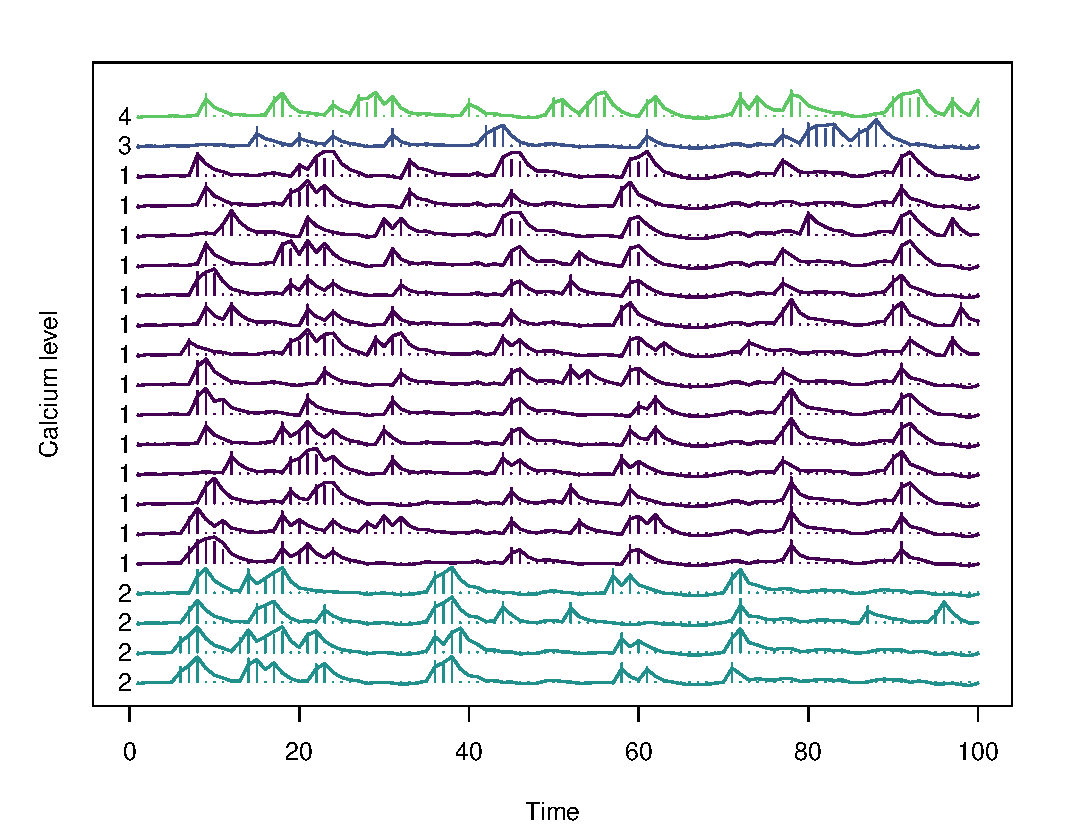
\includegraphics[width=.75\linewidth]{ch4/t100n20}\\
	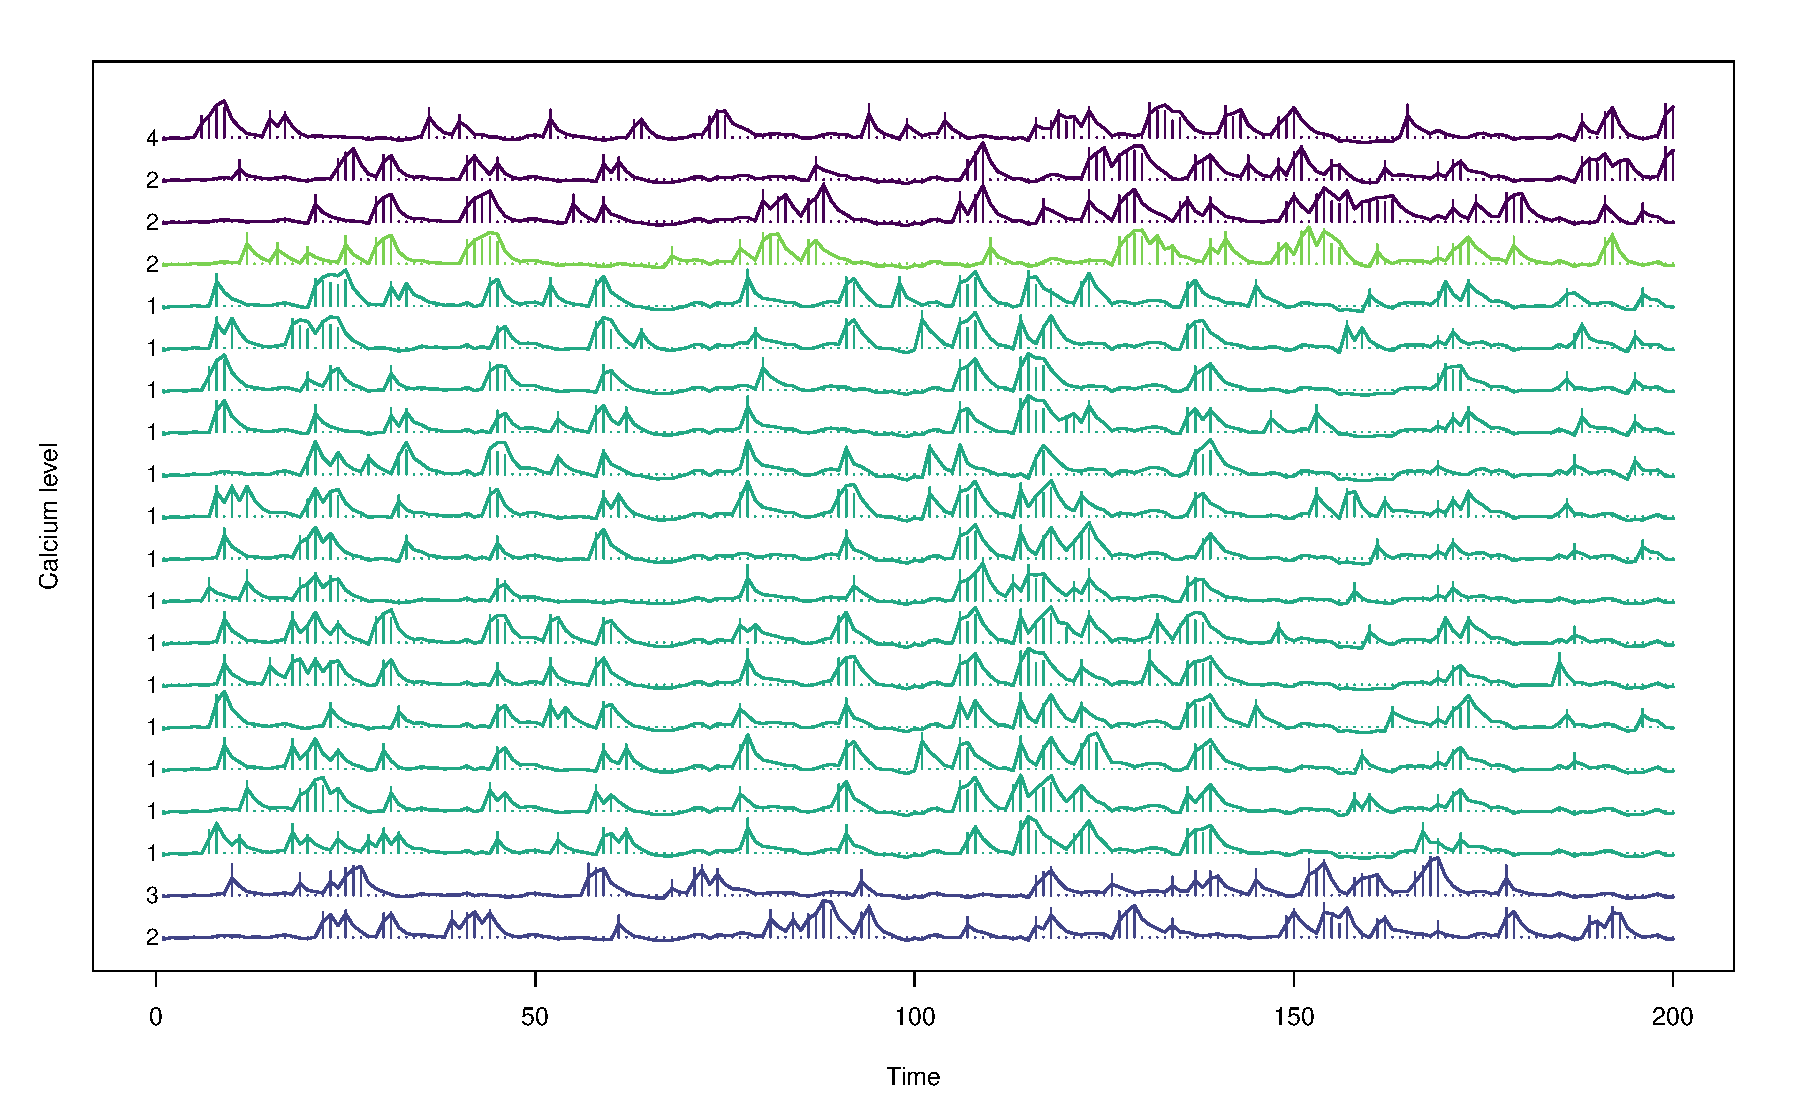
\includegraphics[width=\linewidth]{ch4/t200n20}
	\label{ch4:fig_n20}
	\caption[Estimated clustering on the simulated data with sample size $n=20$.]{Estimated clustering on the simulated data with sample size $n=20$, and series length $T=100$ (left) and $T=200$ (right). The colors correspond to the estimated clusters, while the numbers on the left of each series correspond to the true partition.}
\end{figure}

\begin{figure}
	\centering
	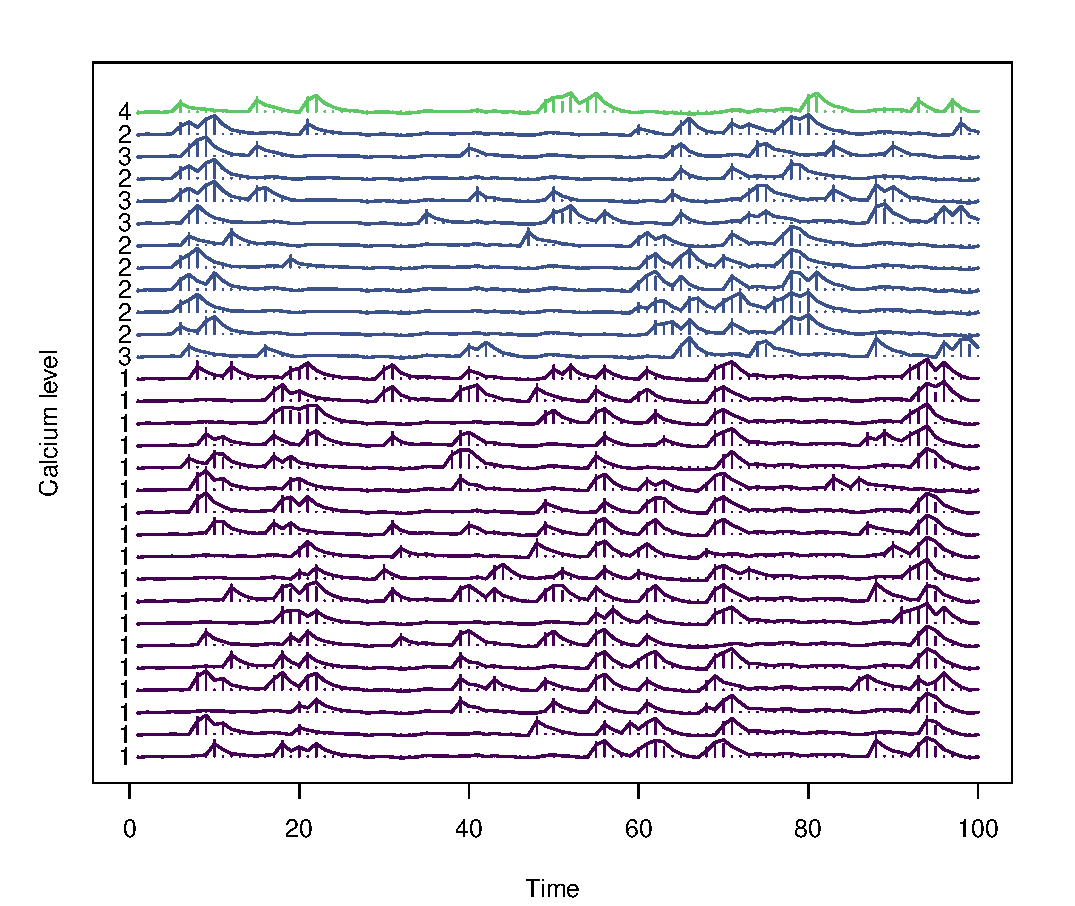
\includegraphics[width=.75\linewidth]{ch4/t100n30}\\
	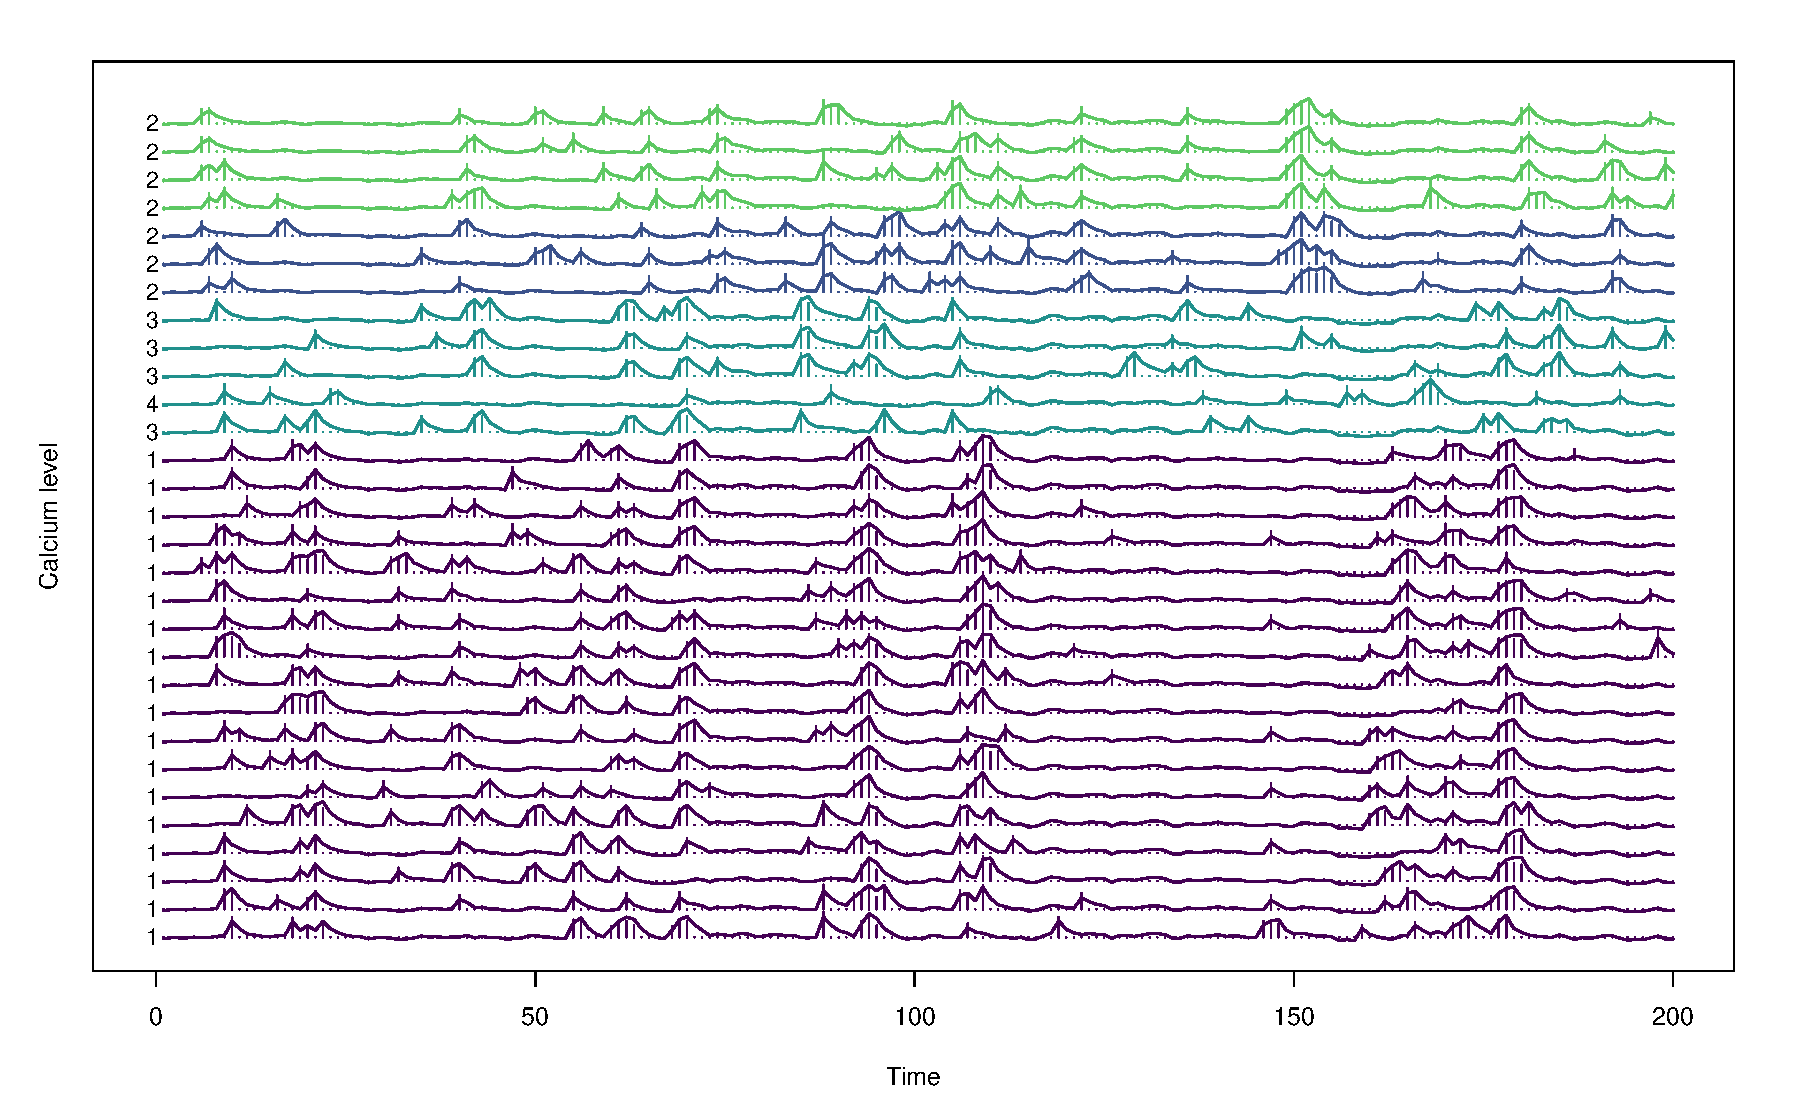
\includegraphics[width=\linewidth]{ch4/t200n30}
	\label{ch4:fig_n30}
	\caption[Estimated clustering on the simulated data with sample size $n=30$.]{Estimated clustering on the simulated data with sample size $n=30$, and series length $T=100$ (left) and $T=200$ (right). The colors correspond to the estimated clusters, while the numbers on the left of each series correspond to the true partition.}
\end{figure}

\begin{figure}
	\centering
	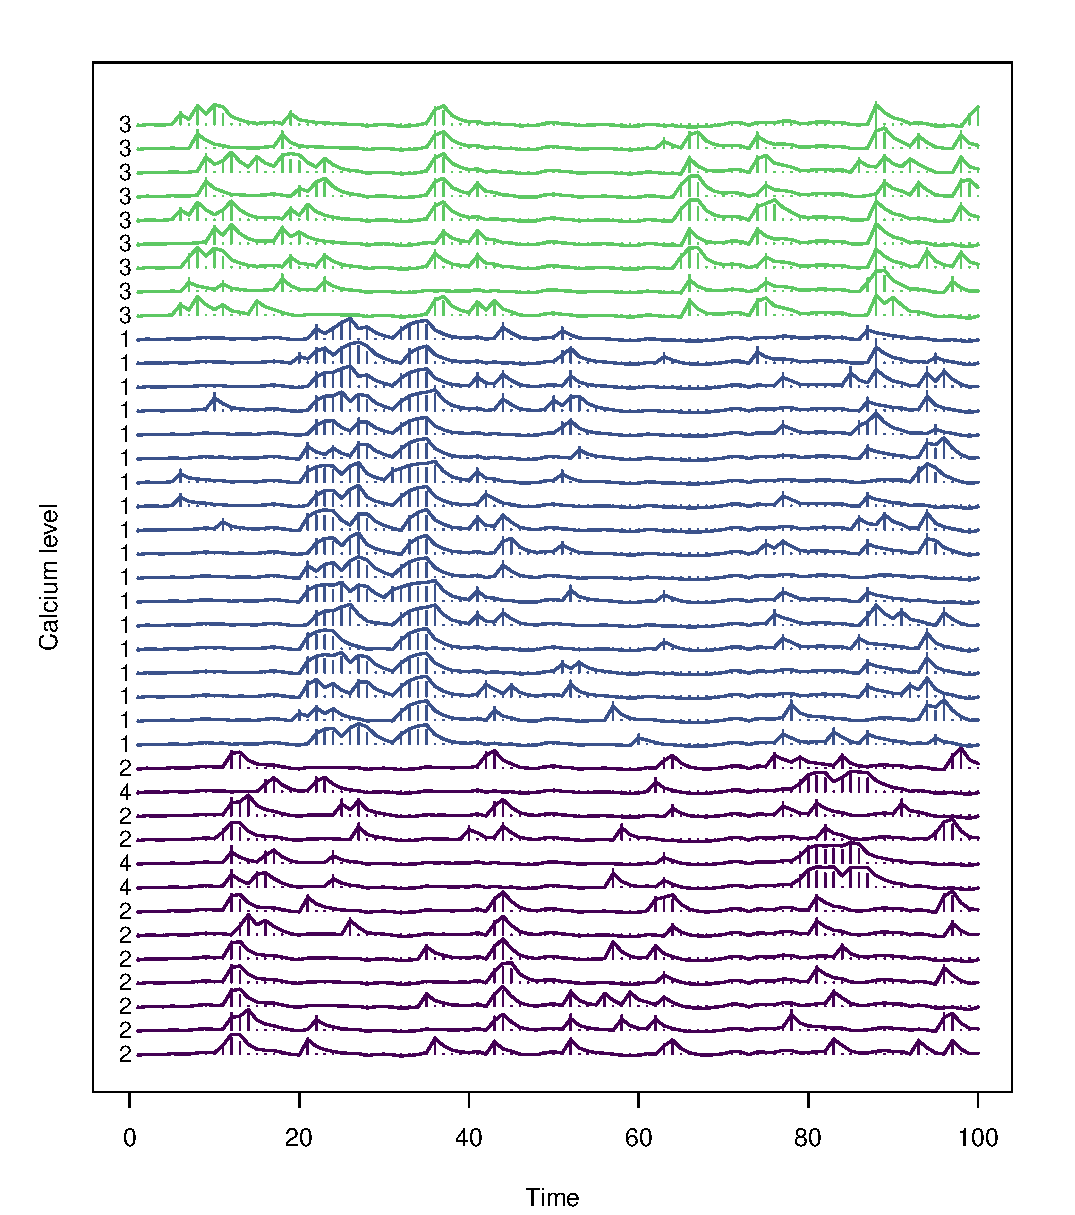
\includegraphics[width=.65\linewidth]{ch4/t100n40}\\
	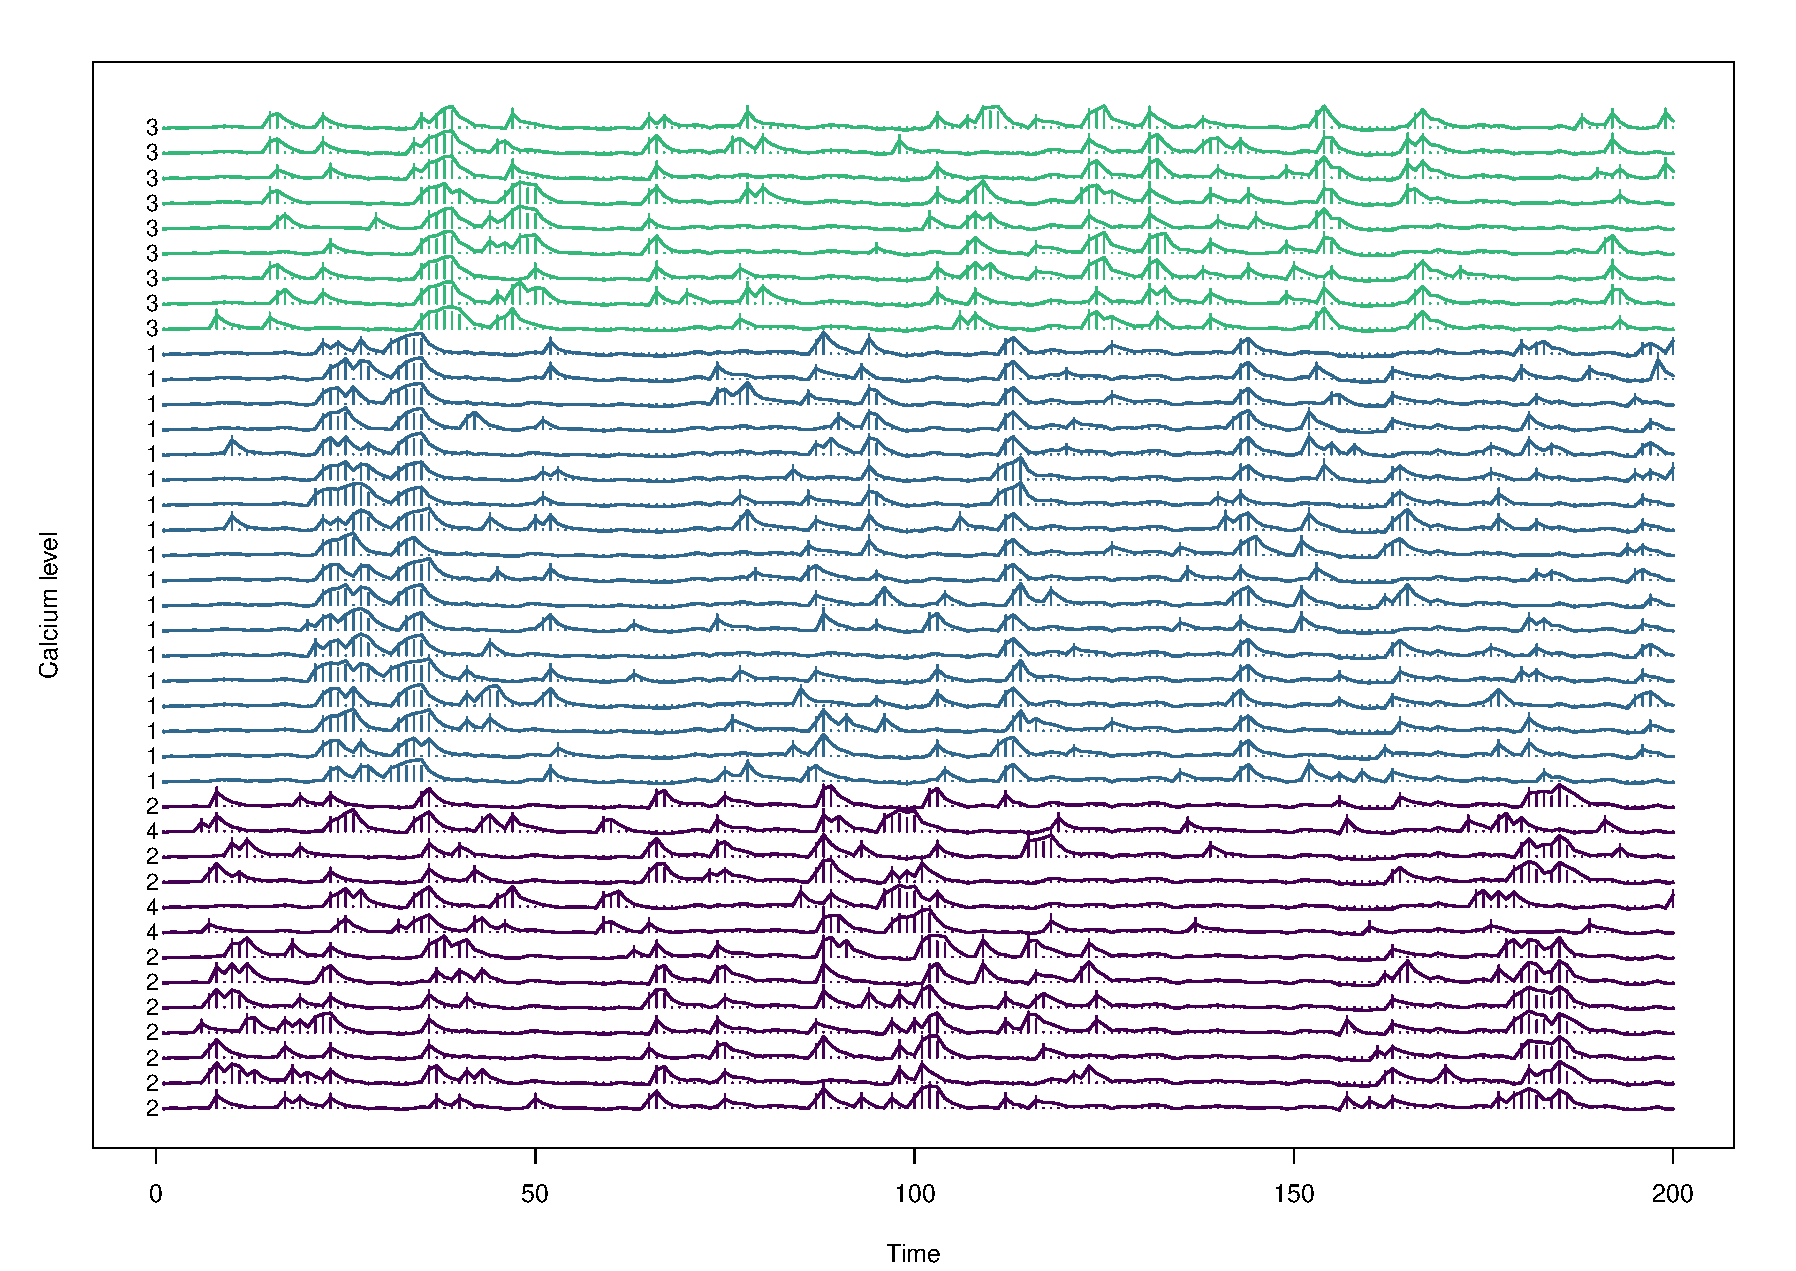
\includegraphics[width=\linewidth]{ch4/t200n40}
	\label{ch4:fig_n40}
	\caption[Estimated clustering on the simulated data with sample size $n=40$.]{Estimated clustering on the simulated data with sample size $n=40$, and series length $T=100$ (left) and $T=200$ (right). The colors correspond to the estimated clusters, while the numbers on the left of each series correspond to the true partition.}
\end{figure}





%\section{Analysis of hippocampal neurons}




